\documentclass[11pt,a4paper]{article}
\usepackage[utf8]{inputenc}
\usepackage[T1]{fontenc}
\usepackage{amsfonts}
\usepackage{amssymb}
\usepackage{mdframed}
\usepackage{tikz}
\usepackage{tkz-tab}
\usepackage{pgfplots}
\usepackage{xcolor}
\usepackage{fancyhdr}
\usepackage{lastpage}
\usepackage[fleqn]{amsmath}
\usepackage{yhmath}
\usepackage{array}
\setlength{\mathindent}{0pt}

% Spécifications du document
\newcommand{\doctitre}{Trigonométrie} % Ex: Le second degré
\newcommand{\docniveau}{$1^{\text{re}}$ Spécialité mathématiques} % Ex: $1^{\text{re}}$ Spécialité mathématiques
\newcommand{\doctheme}{Analyse} %Ex: Algèbre
\newcommand{\doctype}{Cours} % Ex: Démonstrations
\newcommand{\docshorttype}{Cours} % Démo

% Couleurs pour les graphiques
\definecolor{dark_green}{HTML}{008000}

% Paramètres du document
\RequirePackage{geometry}
\geometry{tmargin=1cm,bmargin=1.9cm,lmargin=1.9cm,rmargin=1.9cm}
\renewcommand{\familydefault}{\sfdefault}
\setlength{\parindent}{0pt}
\title{\doctitre}
\author{\docniveau \\ \doctheme\text{ - }\doctype}
\date{}
\fancypagestyle{custom}{
  \fancyhf{}
  \renewcommand{\headrulewidth}{0pt}
  \lfoot{\doctheme\text{ - }\docshorttype}
  \cfoot{\doctitre} % Change \titre to \doctitre
  \rfoot{\thepage/\pageref{LastPage}}
}

% Styles pour les mdframed
\mdfdefinestyle{definitionStyle}{
    leftline=true,
    rightline=false,
    topline=false,
    bottomline=false,
    linewidth=2pt,
    linecolor=black,
    innertopmargin=0pt,
    innerbottommargin=0pt,
    innerrightmargin=0pt,
    innerleftmargin=5pt,
}

\mdfdefinestyle{proprieteStyle}{
    linewidth=1pt,
    linecolor=black,
    innertopmargin=5pt,
    innerbottommargin=5pt,
    innerrightmargin=5pt,
    innerleftmargin=5pt,
}

\newcolumntype{Y}{>{\centering\arraybackslash}m{1.2cm}}


% ----- DEBUT DU DOCUMENT -----
\begin{document}

% Style et numérotation
\maketitle
\pagestyle{custom}
\thispagestyle{custom}

\section*{I. Lecture sur le cercle trigonométrique}

\begin{minipage}{0.4\textwidth}
    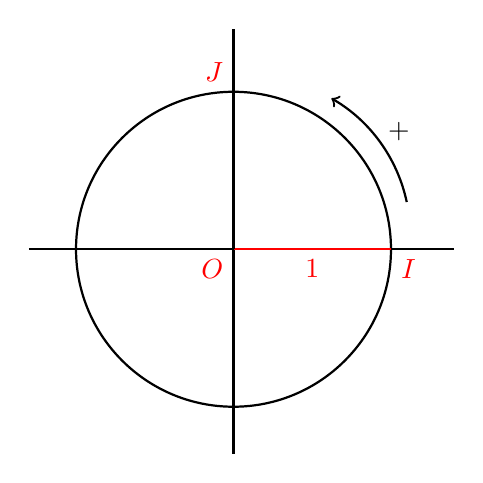
\begin{tikzpicture}[scale=2]
        % Axes
        \draw[thick] (-1.3,0) -- (1.4,0);
        \draw[thick] (0,-1.3) -- (0,1.4);
        % Cercle trigonométrique
        \draw [thick] (0,0) circle (1);
        % Repère (O,I,J)
        \draw [red, thick] (0,0) node[below left] {$O$} -- (1,0) node[below right] {$I$} node[midway,below] {$1$};
        \draw [thick] (0,0) -- (0,1) node[above left] {$\color{red}J$};
        % Angle
        \draw[->, thick] (1.1,0.3) arc (12:60:1);
        \node at (1.05,0.75) {+};
    \end{tikzpicture}
\end{minipage}
\hfill
\begin{minipage}{0.6\textwidth}
    \subsection*{1. Le cercle trigonométrique}
    \begin{mdframed}[style=definitionStyle]
        \textbf{Définition :} ~\\
        Dans un repère orhonormé $(O, I, J)$, le cercle trigonométrique de centre $O$ est le cercle qui a pour rayon $1$ et qui est muni d'un sens direct, le sens trigonométrique.
    \end{mdframed}
    \subsection*{2. Longueur d'un arc et radian}
    \begin{mdframed}[style=proprieteStyle]
        \textbf{Propriété :} ~\\
        Sur un cercle trigonométrique, la longueur de l'arc de cercle $\wideparen{IM}$ (exprimé dans l'unité de longueur du repère), est proportionnelle à la mesure de l'angle $\widehat{OIM}$ exprimé en degrés.
    \end{mdframed}
\end{minipage}
\text{ } \\


\begin{minipage}{0.6\textwidth}
    En effet, le périmètre du cercle est $P=2\pi R=2\pi$. \\ \\
    On a donc
    \renewcommand{\arraystretch}{1.5}
    \begin{tabular}{|c|c|}
        \hline
        $2\pi$           & $360^\circ$     \\ \hline
        $\wideparen{IM}$ & $\widehat{IOM}$ \\ \hline
    \end{tabular}
    car $\displaystyle\wideparen{IM}=\frac{2\pi}{360}\times\widehat{IOM}=\frac{\pi}{180}\times\widehat{IOM}$ \\
\end{minipage}
\hfill
\begin{minipage}{0.3\textwidth}
    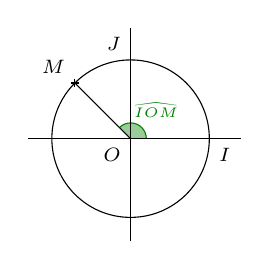
\begin{tikzpicture}[scale=1]
        % Axes
        \draw (-1.3,0) -- (1.4,0);
        \draw (0,-1.3) -- (0,1.4);
        % Cercle trigonométrique
        \draw  (0,0) circle (1);
        % Angle marker
        \draw[dark_green] (0.2,0) arc (0:135:0.2) node[above right] {\tiny{$\text{ }\widehat{IOM}$}};
        \fill[dark_green, opacity=0.4] (0,0) -- (0.2,0) arc (0:135:0.2) -- cycle;
        % Repère (O,I,J)
        \draw (0,0) node[below left] {\scriptsize{$O$}} -- (1,0) node[below right] {\scriptsize{$I$}};
        \draw  (0,0) -- (0,1) node[above left] {\scriptsize{$J$}};
        % Point M
        \node[above left] at (-0.707,0.707) {\scriptsize{$M$}};
        \draw[mark size=1.5pt,mark=+] plot coordinates {(-0.707,0.707)};
        \draw (0,0) -- (-0.707,0.707);
    \end{tikzpicture}
\end{minipage}

\begin{minipage}{0.2\textwidth}
    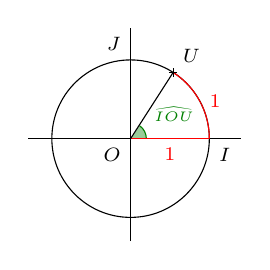
\begin{tikzpicture}[scale=1]
        % Axes
        \draw (-1.3,0) -- (1.4,0);
        \draw (0,-1.3) -- (0,1.4);
        % Cercle trigonométrique
        \draw  (0,0) circle (1);
        % Angle marker
        \draw[dark_green] (0.2,0) arc (0:55:0.2) node[midway,above right] {\tiny{$\widehat{IOU}$}};
        \draw[red] (1,0) arc (0:57:1) node[midway, right] {\scriptsize{$1$}};
        \fill[dark_green, opacity=0.4] (0,0) -- (0.2,0) arc (0:55:0.2) -- cycle;
        % Repère (O,I,J)
        \draw[red] (0,0) node[below left] {\scriptsize{$\color{black}O$}} -- (1,0) node[below right] {\scriptsize{\color{black}$I$}} node[midway,  below] {\scriptsize{$1$}};
        \draw  (0,0) -- (0,1) node[above left] {\scriptsize{$J$}};
        % Point M
        \node[above right] at (0.54,0.84) {\scriptsize{$U$}};
        \draw[mark size=1.5pt,mark=+] plot coordinates {(0.54,0.84)};
        \draw (0,0) -- (0.54,0.84);
    \end{tikzpicture}
\end{minipage}
\hfill
\begin{minipage}{0.8\textwidth}
    \begin{mdframed}[style=definitionStyle]
        \textbf{Définition :} ~\\
        Soit $U$ le point du cercle trigonométrique tel que l'arc $\wideparen{IU}$ ait pour longueur $1$ (exprimé dans l'unité de la longueur du repère). \\
        On définit un radian, noté $1\,\mathrm{rad}$, comme étant la mesure de l'angle $\widehat{IOU}$.
    \end{mdframed}
\end{minipage}
\text{ } ~\\~\\
\textbf{Exemples :$\color{white}\displaystyle{\frac{1}{x}}$} ~\\
\renewcommand{\arraystretch}{1.5}
\begin{tabular}{|l|c|c|c|c|c|c|c|c|c|}
    \hline
    Mesure de l'angle $\widehat{IOM}$ en degrés  & $360$  & $180$ & $90$            & $270$            & $30$            & $45$            & $60$            & $1$               & $\frac{180}{\pi}$ \\ \hline
    Longueur de l'arc $\wideparen{IM}$           & $2\pi$ & $\pi$ & $\frac{\pi}{2}$ & $\frac{3\pi}{2}$ & $\frac{\pi}{6}$ & $\frac{\pi}{4}$ & $\frac{\pi}{3}$ & $\frac{\pi}{180}$ & $1$               \\ \hline
    Mesure de l'angle $\widehat{IOM}$ en radians & $2\pi$ & $\pi$ & $\frac{\pi}{2}$ & $\frac{3\pi}{2}$ & $\frac{\pi}{6}$ & $\frac{\pi}{4}$ & $\frac{\pi}{3}$ & $\frac{\pi}{180}$ & $1$               \\ \hline
\end{tabular}

\newpage

\section*{II. Enroulement de la droite des réels sur le cercle trigonométrique}

Sur le cercle trigonométrique, on choisit un point comme origine et on enroule la droite des réels sur le cercle.

\begin{center}
    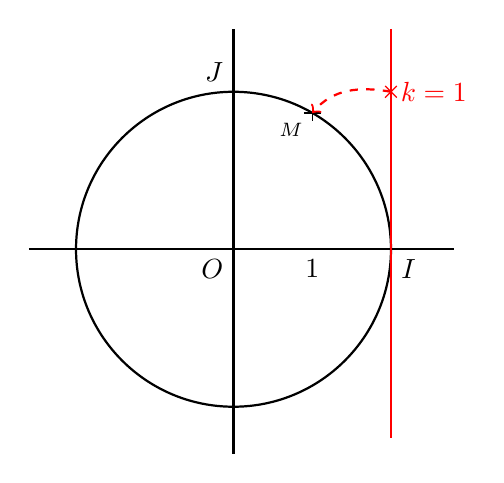
\begin{tikzpicture}[scale=2]
        % Axes
        \draw[thick] (-1.3,0) -- (1.4,0);
        \draw[thick] (0,-1.3) -- (0,1.4);
        % Cercle trigonométrique
        \draw [thick] (0,0) circle (1);
        % Repère (O,I,J)
        \draw [thick] (0,0) node[below left] {$O$} -- (1,0) node[below right] {$I$} node[midway,below] {$1$};
        \draw [thick] (0,0) -- (0,1) node[above left] {$J$};
        % Point M
        \node[below left] at (0.5,0.865) {\scriptsize{$M$}};
        \draw[mark size=1.5pt,mark=+] plot coordinates {(0.5,0.865)};
        % Curved arrow
        \draw[thick, red, dashed, ->] (1,1) to[out=170,in=50] (0.5,0.865);
        % Droite
        \draw[red, thick] (1,1.4) -- (1,-1.2);
        \node[right, red] at (1,1) {$k=1$};
        \draw[red, mark size=1.5pt, mark=x] plot coordinates {(1,1)};
        
    \end{tikzpicture}
\end{center}


\begin{mdframed}[style=proprieteStyle]
    \textbf{Propriétés :}
    \vspace{-4pt}
    \begin{itemize}
        \item En enroulant la droite des réels sur le cercle trigonométrique, on associe à tout réel $x$ un unique point $M$ sur le cercle. \\
              On dit alors que $M$ est l'image de $x$ sur le cercle $C$.
        \item Réciproquement, à tout point $M$ du cercle trigonométrique correspondent une infinité de valeurs qui peuvent être considérés comme les abscisses des points de la droite. \\
              Si $x$ est l'un d'entre eux, les autres abscisses sont $x+2\pi$, $x+4\pi$, $x-2\pi$, $x-4\pi$\dots
    \end{itemize}
\end{mdframed}

\textbf{\\Schéma d'un cercle trigonométrique avec des valeurs remarquables :}
\begin{center}
    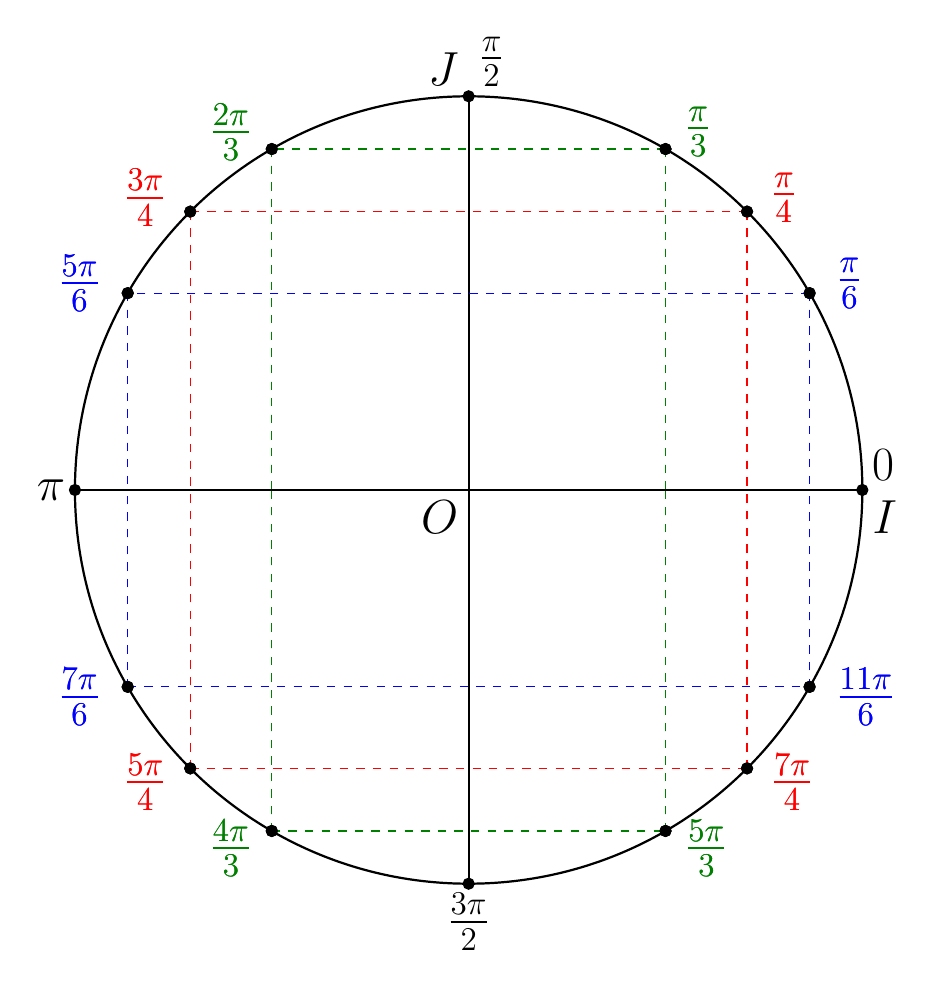
\begin{tikzpicture}[scale=5]
        % Axes
        \draw[thick] (-1,0) -- (1,0) node[right] {};
        \draw[thick] (0,-1) -- (0,1) node[above] {};
        % Cercle trigonométrique
        \draw [thick] (0,0) circle (1);
        % Repère (O,I,J)
        \draw [thick] (0,0) node[below left] {\LARGE{$O$}} -- (1,0) node[below right] {\LARGE{$I$}};
        \draw [thick] (0,0) -- (0,1) node[above left] {\LARGE{$J$}};

        % Points 0
        \node[above right] at (1,0) {\LARGE{$0$}};
        \draw[mark size=0.4pt,mark=*] plot coordinates {(1,0)};
        % Points pi/2
        \node[above right] at (0,1) {\LARGE{$\frac{\pi}{2}$}};
        \draw[mark size=0.4pt,mark=*] plot coordinates {(0,1)};
        % Points pi
        \node[left] at (-1,0) {\LARGE{$\pi$}};
        \draw[mark size=0.4pt,mark=*] plot coordinates {(-1,0)};
        % Points -pi/2
        \node[below] at (0,-1) {\LARGE{$\frac{3\pi}{2}$}};
        \draw[mark size=0.4pt,mark=*] plot coordinates {(0,-1)};

        % Points pi/3
        \foreach \angle/\label/\pos in {60/{$\frac{\pi}{3}$}/right, 120/{$\frac{2\pi}{3}$}/left, 240/{$\frac{4\pi}{3}$}/left, 300/{$\frac{5\pi}{3}$}/right} {
        % Coordonnées polaires (r,θ) pour placer les points
        \coordinate (P\angle) at (\angle:1);
        % Marqueurs de points
        \draw[mark size=0.4pt,mark=*] plot coordinates {(P\angle)};
        % Étiquettes de points
        \path (P\angle) -- ++(\angle:0.05) node[\pos, dark_green] {\LARGE\label};
        % Lignes en pointillés
        \draw[dashed, blue] (P\angle) -- (P\angle |- 0,0);
        \draw[dashed, dark_green] (P\angle) -- (0,0 -| P\angle);
        }
        % Lignes reliant les points
        \draw[dashed, dark_green] (P60) -- (P120);
        \draw[dashed, dark_green] (P240) -- (P300);

        % Points pi/4
        \foreach \angle/\label/\pos in {45/{$\frac{\pi}{4}$}/right, 135/{$\frac{3\pi}{4}$}/left, 225/{$\frac{5\pi}{4}$}/left, 315/{$\frac{7\pi}{4}$}/right} {
        % Coordonnées polaires (r,θ) pour placer les points
        \coordinate (P\angle) at (\angle:1);
        % Marqueurs de points
        \draw[mark size=0.4pt,mark=*] plot coordinates {(P\angle)};
        % Étiquettes de points
        \path (P\angle) -- ++(\angle:0.05) node[\pos, red] {\LARGE\label};
        % Lignes en pointillés
        \draw[dashed, red] (P\angle) -- (P\angle |- 0,0);
        \draw[dashed, red] (P\angle) -- (0,0 -| P\angle);
        }
        % Lignes reliant les points
        \draw[dashed, red] (P45) -- (P135);
        \draw[dashed, red] (P225) -- (P315);

        % Points pi/6
        \foreach \angle/\label/\pos in {30/{$\frac{\pi}{6}$}/right, 150/{$\frac{5\pi}{6}$}/left, 210/{$\frac{7\pi}{6}$}/left, 330/{$\frac{11\pi}{6}$}/right} {
        % Coordonnées polaires (r,θ) pour placer les points
        \coordinate (P\angle) at (\angle:1);
        % Marqueurs de points
        \draw[mark size=0.4pt,mark=*] plot coordinates {(P\angle)};
        % Étiquettes de points
        \path (P\angle) -- ++(\angle:0.05) node[\pos, blue] {\LARGE\label};
        % Lignes en pointillés
        \draw[dashed, blue] (P\angle) -- (P\angle |- 0,0);
        \draw[dashed, blue] (P\angle) -- (0,0 -| P\angle);
        }
        % Lignes reliant les points
        \draw[dashed, blue] (P30) -- (P150);
        \draw[dashed, blue] (P210) -- (P330);

        % Points pi/3
        \foreach \angle/\label/\pos in {60/{$\frac{\pi}{3}$}/right, 120/{$\frac{2\pi}{3}$}/left, 240/{$\frac{4\pi}{3}$}/left, 300/{$\frac{5\pi}{3}$}/right} {
        % Coordonnées polaires (r,θ) pour placer les points
        \coordinate (P\angle) at (\angle:1);
        % Marqueurs de points
        \draw[mark size=0.4pt,mark=*] plot coordinates {(P\angle)};
        % Étiquettes de points
        \path (P\angle) -- ++(\angle:0.05) node[\pos, dark_green] {\LARGE\label};
        }

        % Points pi/4
        \foreach \angle/\label/\pos in {45/{$\frac{\pi}{4}$}/right, 135/{$\frac{3\pi}{4}$}/left, 225/{$\frac{5\pi}{4}$}/left, 315/{$\frac{7\pi}{4}$}/right} {
        % Coordonnées polaires (r,θ) pour placer les points
        \coordinate (P\angle) at (\angle:1);
        % Marqueurs de points
        \draw[mark size=0.4pt,mark=*] plot coordinates {(P\angle)};
        % Étiquettes de points
        \path (P\angle) -- ++(\angle:0.05) node[\pos, red] {\LARGE\label};
        }

        % Points pi/6
        \foreach \angle/\label/\pos in {30/{$\frac{\pi}{6}$}/right, 150/{$\frac{5\pi}{6}$}/left, 210/{$\frac{7\pi}{6}$}/left, 330/{$\frac{11\pi}{6}$}/right} {
        % Coordonnées polaires (r,θ) pour placer les points
        \coordinate (P\angle) at (\angle:1);
        % Marqueurs de points
        \draw[mark size=0.4pt,mark=*] plot coordinates {(P\angle)};
        % Étiquettes de points
        \path (P\angle) -- ++(\angle:0.05) node[\pos, blue] {\LARGE\label};
        }

    \end{tikzpicture}
\end{center}

\newpage

\section*{III. Cosinus et sinus d'un nombre réel}
\subsection*{1. Définitions}
\begin{mdframed}[style=definitionStyle]
    \textbf{Définitions :} ~\\
    $C$ est le cercle trigonométrique de centre $O$ et $(O,I,J)$ un repère orhonormé direct. $x$ est un nombre réel et $M$ est le points image du réel $x$ sur le cercle trigonométrique.
    \begin{itemize}
        \item Le cosinus de $x$, noté $\cos{x}$, est l'abscisse de $M$ dans le repère $(O,I,J)$.
        \item Le sinus de $x$, noté $\sin{x}$, est l'ordonnée de $M$ dans le repère $(O,I,J)$.
    \end{itemize}
\end{mdframed}

\begin{minipage}{0.6\textwidth}
    \begin{mdframed}[style=proprieteStyle]
        \textbf{Propriétés :} ~\\
        Pour tout réel $x$ et tout entier relatif $k$, on a :
        \begin{itemize}
            \item $\cos^2{x}+\sin^2{x}=1$
            \item $\cos(x+2k\pi)=\cos{x}$
            \item $-1\leq\cos{x}\leq1$
            \item $-1\leq\sin{x}\leq1$
        \end{itemize}
    \end{mdframed}
\end{minipage}
\hfill
\begin{minipage}{0.3\textwidth}
    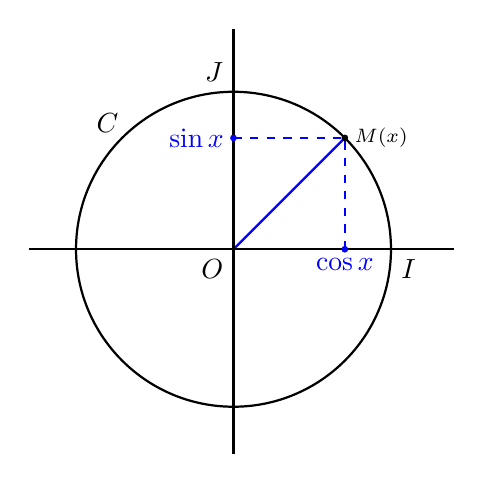
\begin{tikzpicture}[scale=2]
        % Cercle trigonométrique
        \draw [thick] (0,0) circle (1);
        % Repère (O,I,J)
        \draw [thick] (0,0) node[below left] {$O$} -- (1,0) node[below right] {$I$};
        \draw [thick] (0,0) -- (0,1) node[above left] {$J$};
        \node at (-0.8,0.8) {$C$};
        % Point M
        \node[right] at (0.707,0.707) {\scriptsize{$M(x)$}};
        \node[blue,mark size=0.4pt,mark=*, below] at (0.707, 0) {$\cos{x}$};
        \node[blue, left] at (0, 0.707) {$\sin{x}$};
        \draw[blue, thick] (0,0) -- (0.707,0.707) node[midway, above left] {};
        \draw[blue, thick, dashed] (0.707,0) -- (0.707,0.707) node[midway, above left] {};
        \draw[blue, thick, dashed] (0,0.707) -- (0.707,0.707) node[midway, above left] {};
        \draw[mark size=0.5pt,mark=*] plot coordinates {(0.707,0.707)};
        % Axes
        \draw[thick] (-1.3,0) -- (1.4,0);
        \draw[thick] (0,-1.3) -- (0,1.4);
        \draw[blue, mark size=0.5pt,mark=*] plot coordinates {(0.707,0)};
        \draw[blue, mark size=0.5pt,mark=*] plot coordinates {(0,0.707)};
    \end{tikzpicture}
\end{minipage}

\subsection*{2. Valeurs remarquables du cosinus et du sinus}

\renewcommand{\arraystretch}{2.5}
\begin{tabular}{|Y|Y|Y|Y|Y|Y|}
    \hline
    \large{$x$}       & \Large{$0$} & \Large{$\frac{\pi}{2}$} & \Large{$\frac{\pi}{3}$}      & \Large{$\frac{\pi}{4}$}      & \Large{$\frac{\pi}{6}$}      \\
    \hline
    \large{$\cos{x}$} & \Large{$1$} & \Large{$0$}             & \Large{$\frac{1}{2}$}        & \Large{$\frac{\sqrt{2}}{2}$} & \Large{$\frac{\sqrt{3}}{2}$} \\
    \hline
    \large{$\sin{x}$} & \Large{$0$} & \Large{$1$}             & \Large{$\frac{\sqrt{3}}{2}$} & \Large{$\frac{\sqrt{2}}{2}$} & \Large{$\frac{1}{2}$}        \\
    \hline
\end{tabular}

\subsection*{3. Lien avec le cosinus et sinus dans un triangle rectangle}


\begin{minipage}{0.6\textwidth}
    On considère le cercle trigonométrique et la tangente $D$ au cercle. \\
    Soit $x\in]0;\frac{\pi}{2}[$ et $M$ son point image. \\
                Soit $H$ le projeté orhogonal de $M$ sur $(OI)$. \\
                Soit $H'$ le projeté orhogonal de $M$ sur $(OJ)$. \\

                On a alors : \\
            $\cos(\widehat{IOM})=\frac{\text{côtés adjacents}}{\text{hypoténuse}}=\frac{OH}{OM}=\frac{OH}{1}=OH=\cos{x}$ \\
            $\sin(\widehat{IOM})=\frac{\text{côtés opposé}}{\text{hypoténuse}}=\frac{HM}{OM}=\frac{HM}{1}=OH'=\sin{x}$ \\

                La notion de cosinus et de sinus d'un réel de l'intervalle $]0;\frac{\pi}{2}[$ \\
    coïncident avec les notions de cosinus et sinus d'angle aigu vues \\ aux  collège.
\end{minipage}
\hfill
\begin{minipage}{0.4\textwidth}
    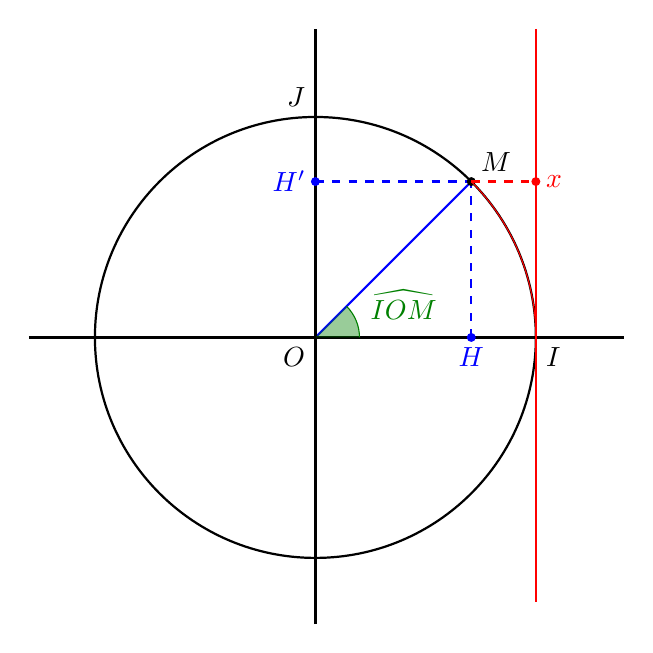
\begin{tikzpicture}[scale=2.8]
        % Cercle trigonométrique
        \draw [thick] (0,0) circle (1);
        % Repère (O,I,J)
        \draw [thick] (0,0) node[below left] {$O$} -- (1,0) node[below right] {$I$};
        \draw [thick] (0,0) -- (0,1) node[above left] {$J$};
        % Point M
        \node[above right] at (0.707,0.707) {$M$};
        \node[blue,mark size=0.4pt,mark=*, below] at (0.707, 0) {$H$};
        \node[blue, left] at (0, 0.707) {$H'$};
        \draw[blue, thick] (0,0) -- (0.707,0.707) node[midway, above left] {};
        \draw[blue, thick, dashed] (0.707,0) -- (0.707,0.707) node[midway, above left] {};
        \draw[blue, thick, dashed] (0,0.707) -- (0.707,0.707) node[midway, above left] {};
        \draw[mark size=0.5pt,mark=*] plot coordinates {(0.707,0.707)};
        % Axes
        \draw[thick] (-1.3,0) -- (1.4,0);
        \draw[thick] (0,-1.3) -- (0,1.4);
        \draw[blue, mark size=0.5pt,mark=*] plot coordinates {(0.707,0)};
        \draw[blue, mark size=0.5pt,mark=*] plot coordinates {(0,0.707)};
        % Droite
        \draw[red, thick] (1,1.4) -- (1,-1.2);
        \draw[red, thick, dashed] (0.707,0.707) -- (1,0.707) node[right] {$x$};
        \draw[red, mark size=0.5pt,mark=*] plot coordinates {(1,0.707)};

        % Angle marker
        \node[dark_green] at (0.4,0.15) {$\widehat{IOM}$};
        \draw[dark_green] (0.2,0) arc (0:45:0.2) {};
        \draw[red] (1,0) arc (0:45:1) node[midway, right] {};
        \fill[dark_green, opacity=0.4] (0,0) -- (0.2,0) arc (0:45:0.2) -- cycle;

    \end{tikzpicture}
\end{minipage}

\newpage

\section*{IV. Fonctions cosinus et sinus}

\begin{mdframed}[style=definitionStyle]
    \textbf{Définitions :}
    \vspace{-4pt}
    \begin{itemize}
        \item On appelle fonction cosinus la fonction notée $\cos$ définie sur $\mathbb{R}$ par $\cos:x\mapsto\cos x$.
        \item On appelle fonction sinus la fonction notée $\sin$ définie sur $\mathbb{R}$ par $\sin:x\mapsto\sin x$.
    \end{itemize}
\end{mdframed}

\begin{mdframed}[style=proprieteStyle]
    \textbf{Propriété :} ~\\
    Pour tout réel $x$, $\cos(-x)=\cos{x}$ et $\sin(-x)=-\sin{x}$. \\
    Ainsi, la fonction cosinus est paire et la fonction sinus est impaire.
\end{mdframed}

\textbf{Conséquences graphique :}
\vspace{-4pt}
\begin{itemize}
    \item La courbe représentative de la fonction $\cos$ est symétrique par rapport à l'axe des ordonnées.
    \item La courbe représentative de la fonction $\sin$ est symétrique par rapport à l'origine du repère.
\end{itemize}

\begin{mdframed}[style=proprieteStyle]
    \textbf{Propriété :} ~\\
    Pour tout réel $x$, $\cos{x}=\cos(x+2\pi)$ et $\sin{x}=\sin(x+2\pi)$.\\
    On dit que les fonctions cosinus et sinus sont des fonction périodiques de période $2\pi$.
\end{mdframed}

\textbf{Conséquence graphique :} ~\\
Les courbes représentatives de la fonction cosinus et sinus se reproduisent identiques à elles-mêmes sur un intervalle de longueur $2\pi$.

\begin{mdframed}[style=proprieteStyle]
    \textbf{Propriété \emph{(variations des fonctions cosinus et sinus)}:} ~\\
    Les deux propriétés précédentes nous permettent de réduire l'intervalle d'étude des deux fonctions $\cos$ et $\sin$ à l'intervalle $[0;\pi]$. \\

    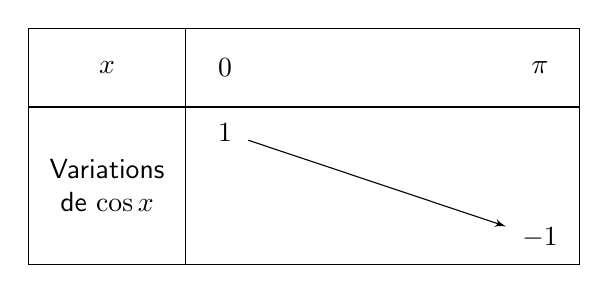
\begin{tikzpicture}
        \tkzTabInit[espcl=4]{$x$ / 1, Variations de $\cos{x}$ / 2}{$0$, $\pi$}
        \tkzTabVar{+/ $1$, -/$-1$ }
    \end{tikzpicture}
    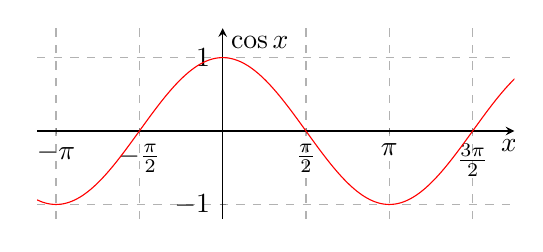
\begin{tikzpicture}[scale=0.5]
        \begin{axis}[
                axis lines=middle,
                xtick={-3.1416, -1.5708, 1.5708, 3.1416, 4.7124, 6.2832},
                xticklabels={$-\pi$, $-\frac{\pi}{2}$, $\frac{\pi}{2}$, $\pi$, $\frac{3\pi}{2}$},
                ytick={-1,0,1},
                ymin=-1.2, ymax=1.4,
                xmin=-3.5, xmax=5.5,
                grid=major,
                grid style={dashed,black!30},
                width=\textwidth,
                height=0.4\textwidth,
                scale only axis,
                axis line style={->, >=stealth},
                set layers
            ]
            \addplot[red,smooth,samples=200,domain=-3.5:6.5] {cos(deg(x))};
            \node at (axis cs:0.7,1.2) {$\cos{x}$};
            \node at (axis cs:5.4,-0.2) {$x$};
        \end{axis}
    \end{tikzpicture}

    \text{ }

    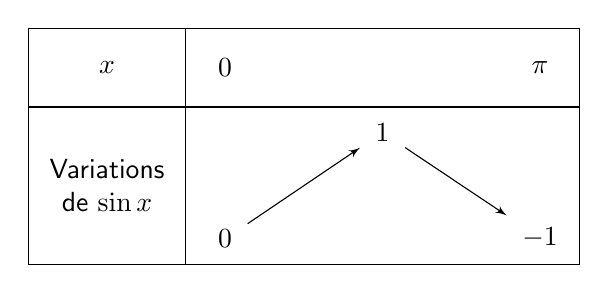
\begin{tikzpicture}
        \tkzTabInit[espcl=2]{$x$ / 1, Variations de $\sin{x}$ /2}{$0$, $ $, $\pi$}
        \tkzTabVar{-/ $0$, +/$1$, -/$-1$ }
    \end{tikzpicture}
    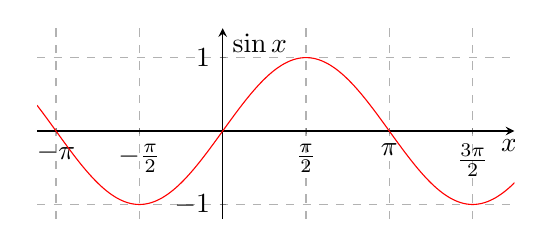
\begin{tikzpicture}[scale=0.5]
        \begin{axis}[
                axis lines=middle,
                xtick={-3.1416, -1.5708, 1.5708, 3.1416, 4.7124},
                xticklabels={$-\pi$, $-\frac{\pi}{2}$, $\frac{\pi}{2}$, $\pi$, $\frac{3\pi}{2}$},
                ytick={-1,0,1},
                ymin=-1.2, ymax=1.4,
                xmin=-3.5, xmax=5.5,
                grid=major,
                grid style={dashed,black!30},
                width=\textwidth,
                height=0.4\textwidth,
                scale only axis,
                axis line style={->, >=stealth},
                set layers
            ]
            \addplot[red,smooth,samples=200,domain=-3.5:6.5] {sin(deg(x))};
            \node at (axis cs:0.7,1.2) {$\sin{x}$};
            \node at (axis cs:5.4,-0.2) {$x$};
        \end{axis}
    \end{tikzpicture}

\end{mdframed}

\end{document}
% ----- FIN DU DOCUMENT -----